%
% IAT 267: Introduction to Technological Systems - A Course Overview
% Section: Networking
%
% Author: Jeffrey Leung
%

\section{Networking}
	\label{sec:networking}
\subsection{Overview}
	\label{subsec:networking:overview}
\begin{easylist}

	& Allows connections between remote devices and systems

	& \emph{Client:} Device which requests the server and receives a reply
	& \emph{Server:} Device which returns information in response to a client's request
	
	& Identification of a device in a network generally requires an address and a port
		&& \emph{Address:} Unique identification of a device in a network
			&&& Communication over the Internet uses IP addresses
		&& \emph{Port:} Virtual point of communciation unique to a given device for information input/output
		&& \emph{Addressing scheme:} Organization and standard for locating devices in a network

	& \emph{Socket:} Endpoint of a data stream in a network
	& \emph{Packet:} Small package of data sent over a network

\end{easylist}
\subsection{Characteristics}
	\label{subsec:networking:characteristics}
\begin{easylist}

	& Layers of connection:
		&& Physical: Devices and connections used
		&& Electrical: Voltage levels which represent data
		&& Logical: Interpretation of voltage levels as data
		&& Data: Timing and grouping of bitwise communication
		&& Application: Arrangement of raw bits into information
		&& Transportation: Sending of information packets to their destination

	& Format and amount of data exchanged:
		&& Congestion of data input
		&& Security of communication
		&& Reception of data in the correct order
		&& Reliability of connection

\end{easylist}
\subsection{Types of Communication}
	\label{subsec:networking:types-of-communication}
\begin{easylist}

	& Clock synchronization:
		&& \emph{Synchronous communication:} Communication between devices which operate on the same, synchronized clock
			&&& Connection is continual
			&&& Used for communication which is time-sensitive
			&&& E.g. Real-time computer games
		&& \emph{Asynchronous communication:} Communication between devices which operate on their own independent clocks
			&&& Connection is created, a request is made, then the connection is closed
			&&& Used for communication which is not time-sensitive
			&&& E.g. Accessing a website
			
	& Communication structure:
		&& \emph{Peer-to-peer model:} Communication between equivalently privileged devices
		&& \emph{Client/server model:} Communication between devices where the client device sends requests to the server device, and the server device shares its resources by providing information

\end{easylist}
\subsection{Network Maps}
	\label{subsec:networking:network-maps}
\begin{easylist}

	& \emph{Network map:} Physical arrangement of connections representing a network

	& Types of network maps:
		&& \emph{Directly connected network:} Network where devices communicate directly
			&&& See figure~\ref{fig:diagram-network-direct} for a diagram
			
			\begin{figure}[!htb]
				\centering
				\href
				{http://www.conceptdraw.com/How-To-Guide/fully-connected-network-topology}
				{
					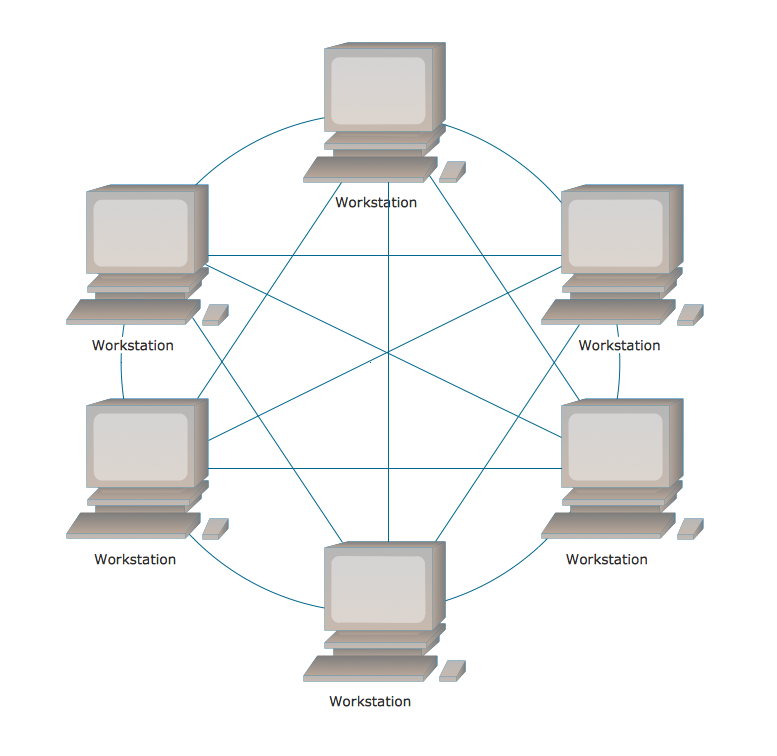
\includegraphics[width=25em]{network-direct}
				}
				\caption{Diagram of a Directly Connected Network}
				\label{fig:diagram-network-direct}
			\end{figure}
			
		&& \emph{Star network:} Network where devices communicate through a single, central device
			&&& See figure~\ref{fig:diagram-network-star} for a diagram
			
			\begin{figure}[!htb]
				\centering
				\href
				{http://starnetworking.weebly.com/}
				{
					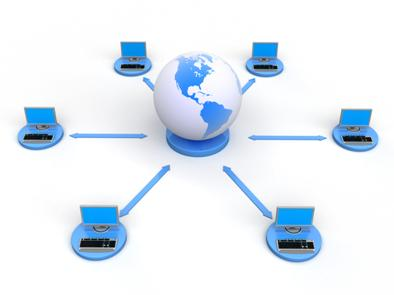
\includegraphics[width=25em]{network-star}
				}
				\caption{Diagram of a Star Network}
				\label{fig:diagram-network-star}
			\end{figure}
			
		&& \emph{Ring network:} Network where devices can communicate directly to two others in order to access another device, such that the devices are connected in a circle
			&&& See figure~\ref{fig:diagram-network-ring} for a diagram
			
			\begin{figure}[!htb]
				\centering
				\href
				{http://www.conceptdraw.com/examples/ring-network-topology}
				{
					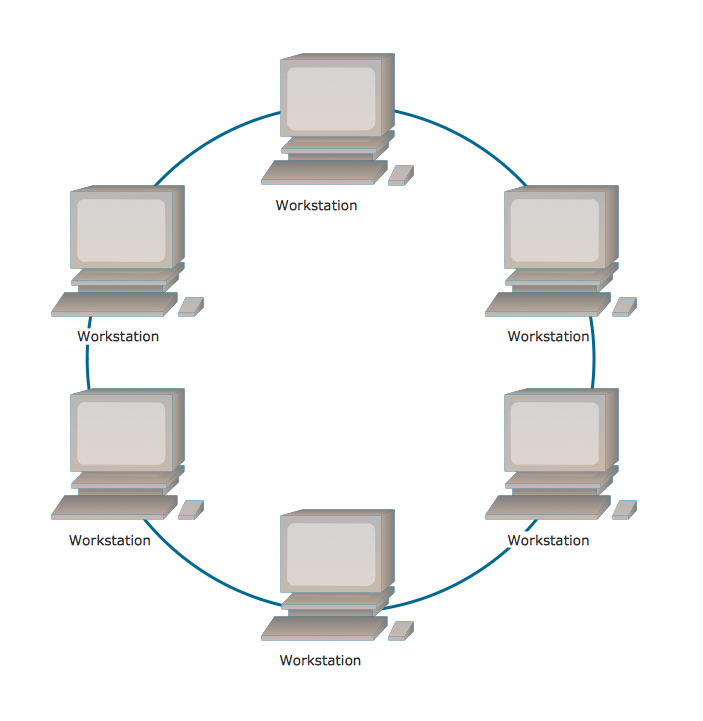
\includegraphics[width=25em]{network-ring}
				}
				\caption{Diagram of a Ring Network}
				\label{fig:diagram-network-ring}
			\end{figure}

\end{easylist}
\subsection{Internet Protocols}
	\label{subsec:networking:internet-protocols}
\begin{easylist}

	& World Wide Web:
		&& Collection of many networks
		&& Uses a network map to keep track of servers and their addresses
	
	& \emph{Socket address:} Unique identifier of a sender or receiver of data on the Internet, consisting of an \hyperref[subsec:networking:characteristics]{IP address} and a \hyperref[subsec:networking:characteristics]{port}
		&& When choosing a custom port in a computer application:
			&&& Common valid port numbers: 0 -- 65536
			&&& Ports reserved for other services: 0 -- 1024
			
	& \emph{User Datagram Protocol (UDP):} Internet communication protocol which is quick and lightweight
		&& Minimal protocol
		&& Does not require confirmation of connection or data transfer (no guarantee of reception)
		&& Order of data is not guaranteed
		&& Useful for time-sensitive information
		
	& \emph{Transmission Control Protocol (TCP):} Internet communication protocol which is reliable and error-checked
		&& Requires confirmation of connection and data transfer
		&& Order of data is guaranteed
		&& Data transmission adapts to the availability of the receiving buffer
		&& Can adapt to a congested network
		
\end{easylist}
\clearpage
